%!TEX root = ../thesis.tex

\newpage
\section{ Графические материалы}
\label{c:graphs}

\setcounter{figure}{0}

\begin{figure}[H]
	\center{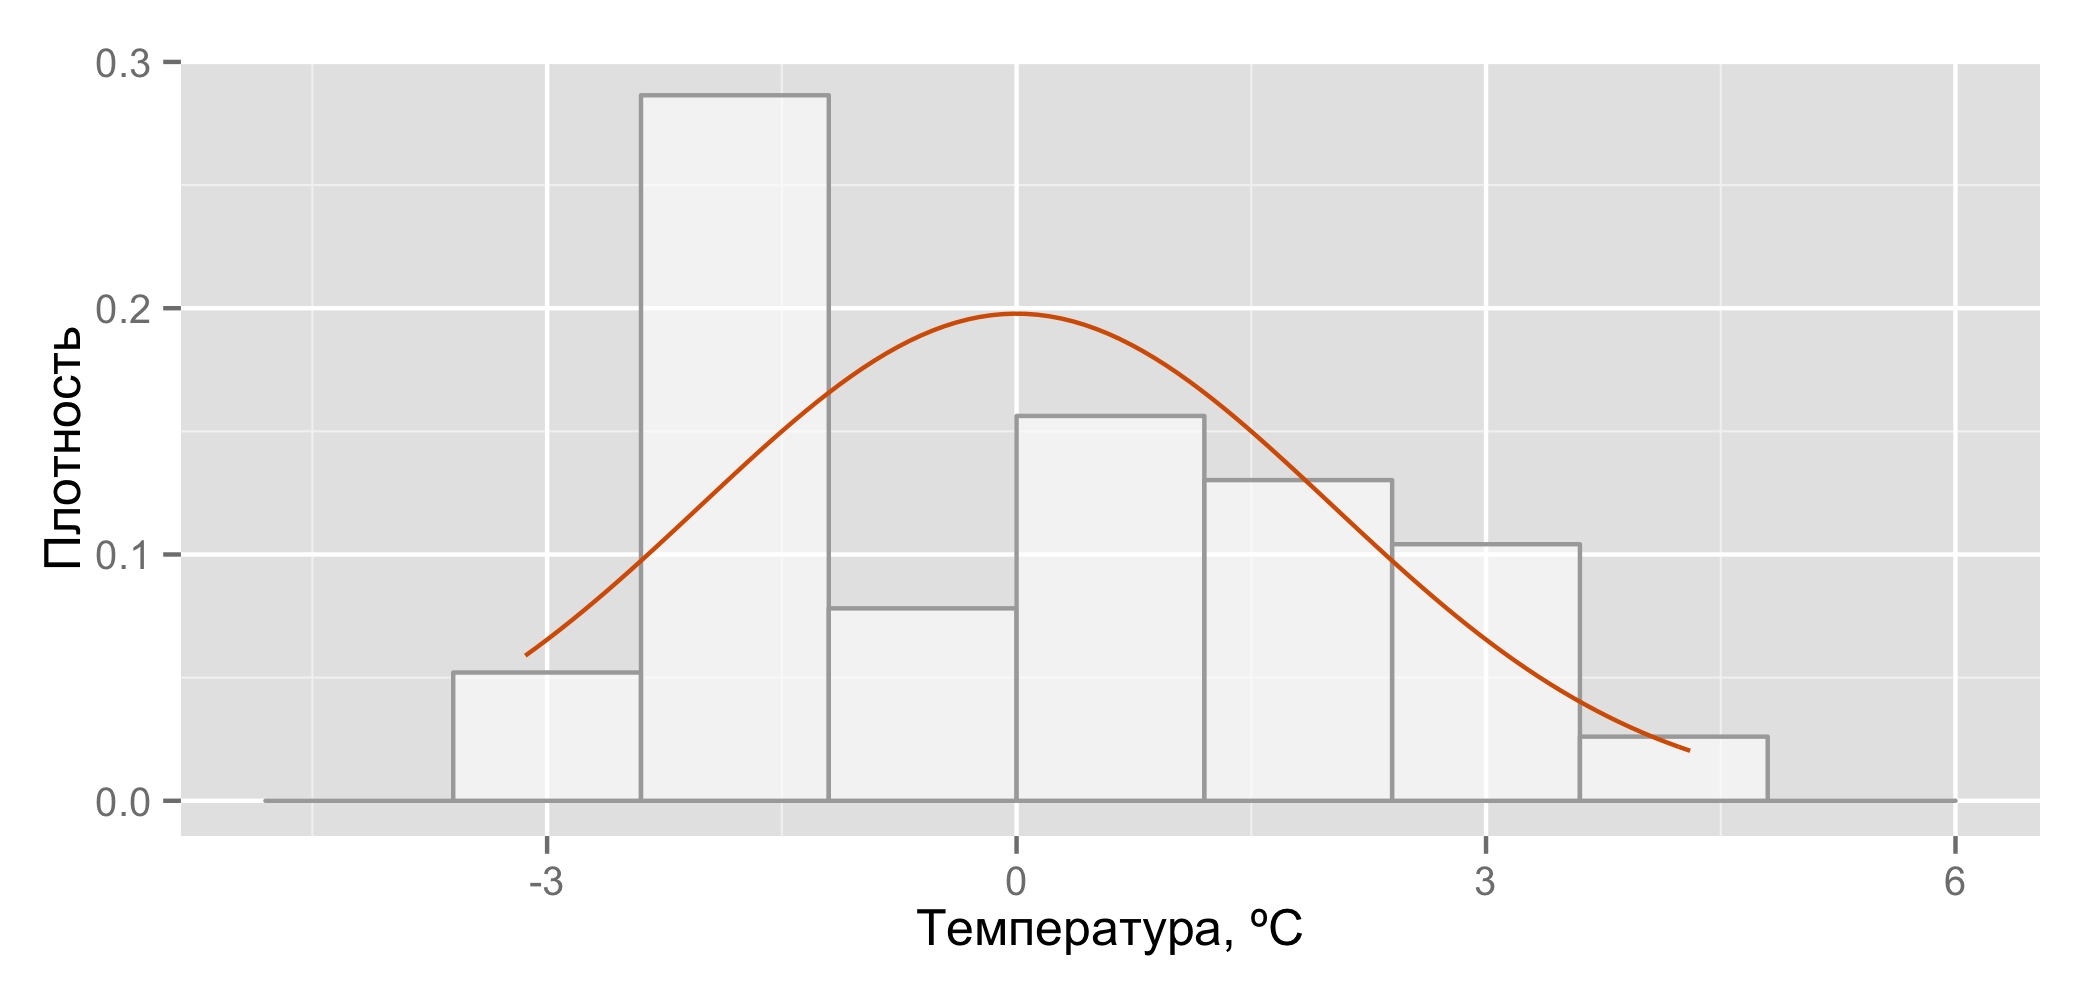
\includegraphics[width=0.9\linewidth]{../figures/residual/histogram.png}}
\caption{Гистограмма остатков с кривой плотности нормального распределения $\mathcal{N}(19.88, 4.92)$}
\label{img:resid_hist}
\end{figure}

\begin{figure}[H]
	\center{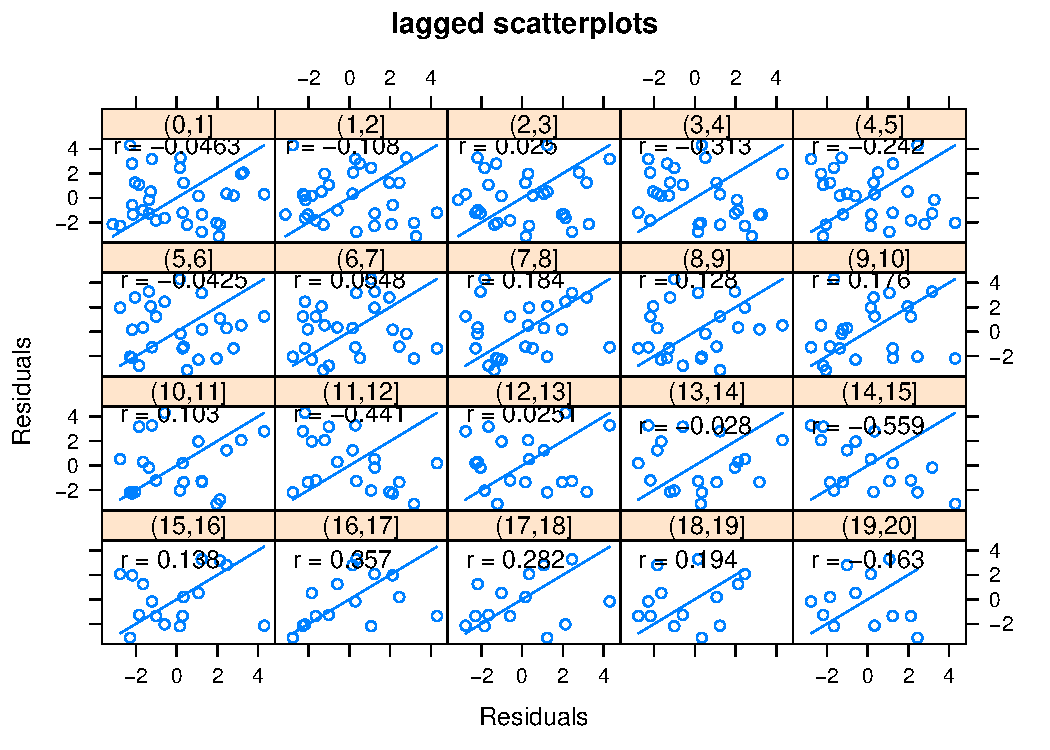
\includegraphics[width=0.9\linewidth]{../figures/residual/hscat.pdf}}
\caption{Диаграмма взаимного разброса}
\label{img:hscat}
\end{figure}

\begin{figure}[H]
	\center{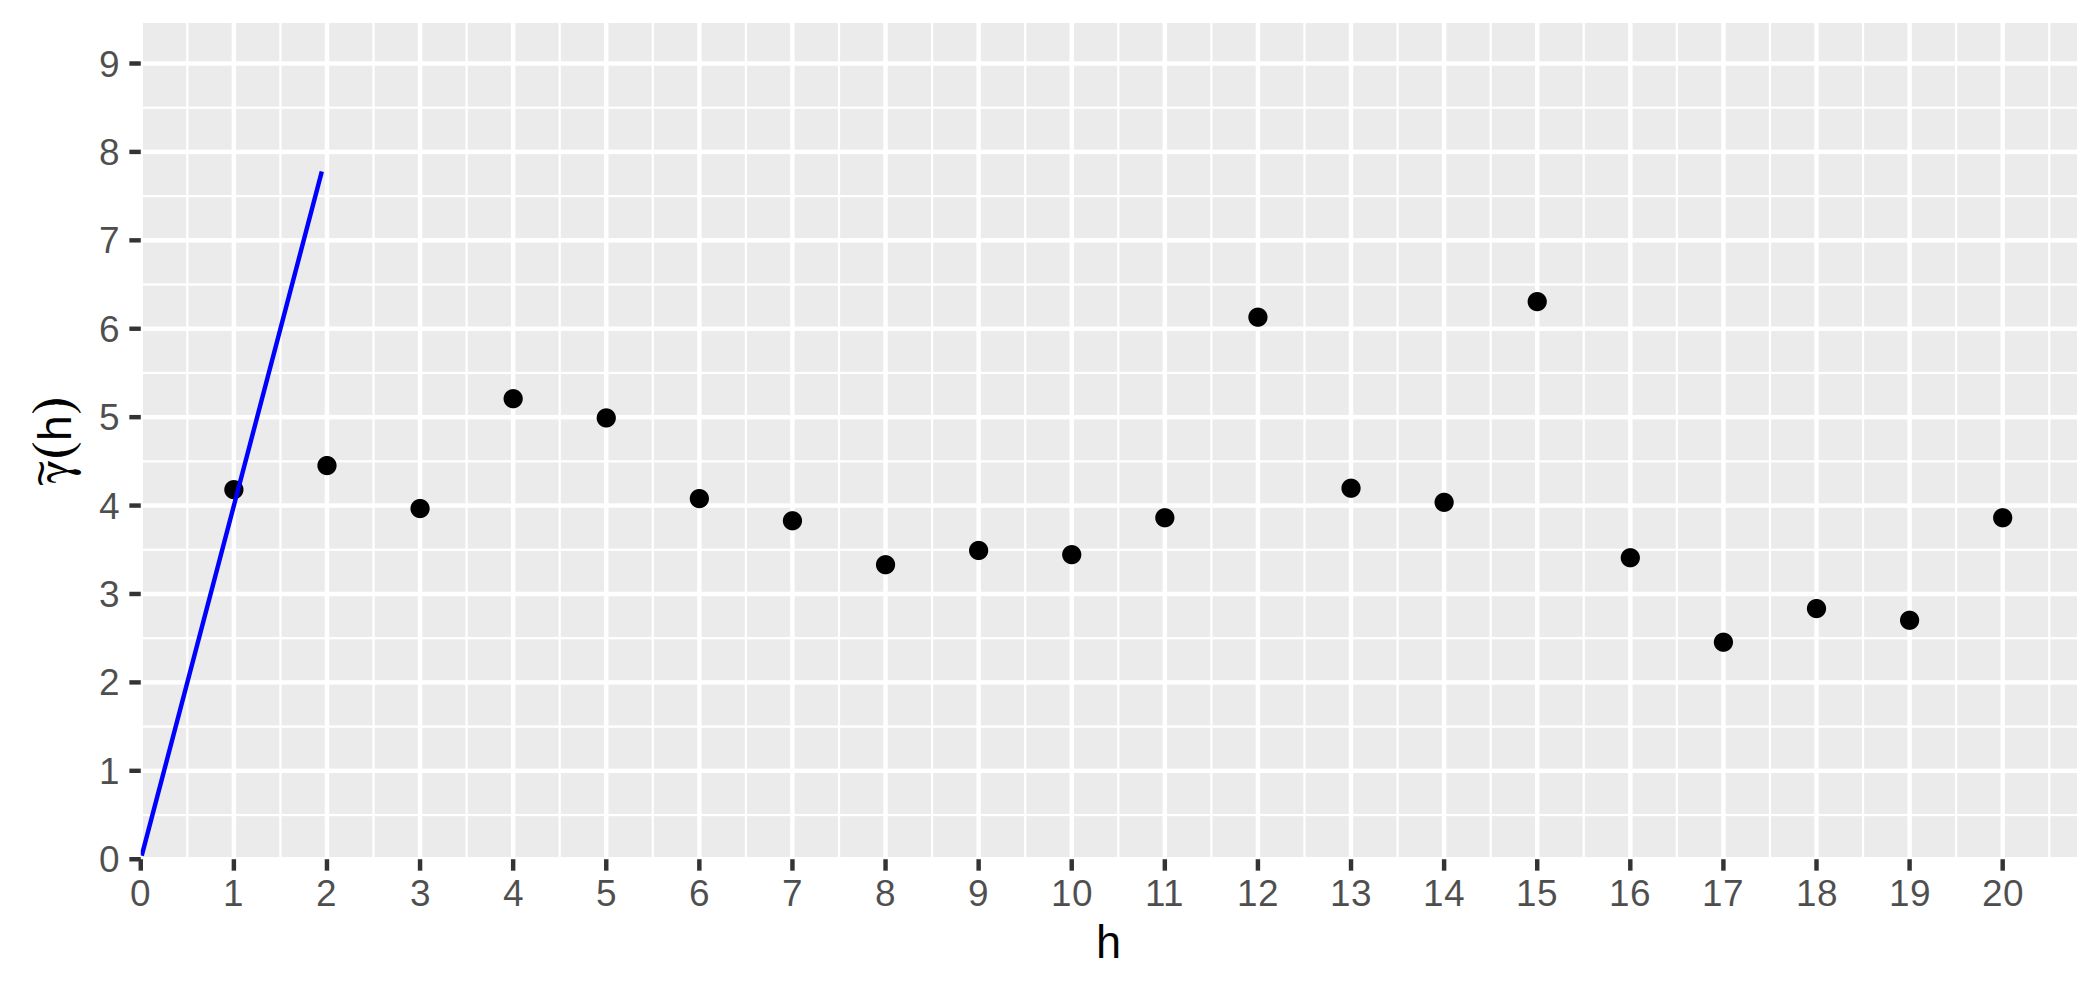
\includegraphics[width=0.8\linewidth]{../figures/variogram/lin-modeled.png}}
\caption{Семивариограмма и оценка $ \widehat{\gamma}_1(h) $}
\label{img:lin-modeled}
\end{figure}

\begin{figure}[H]
	\center{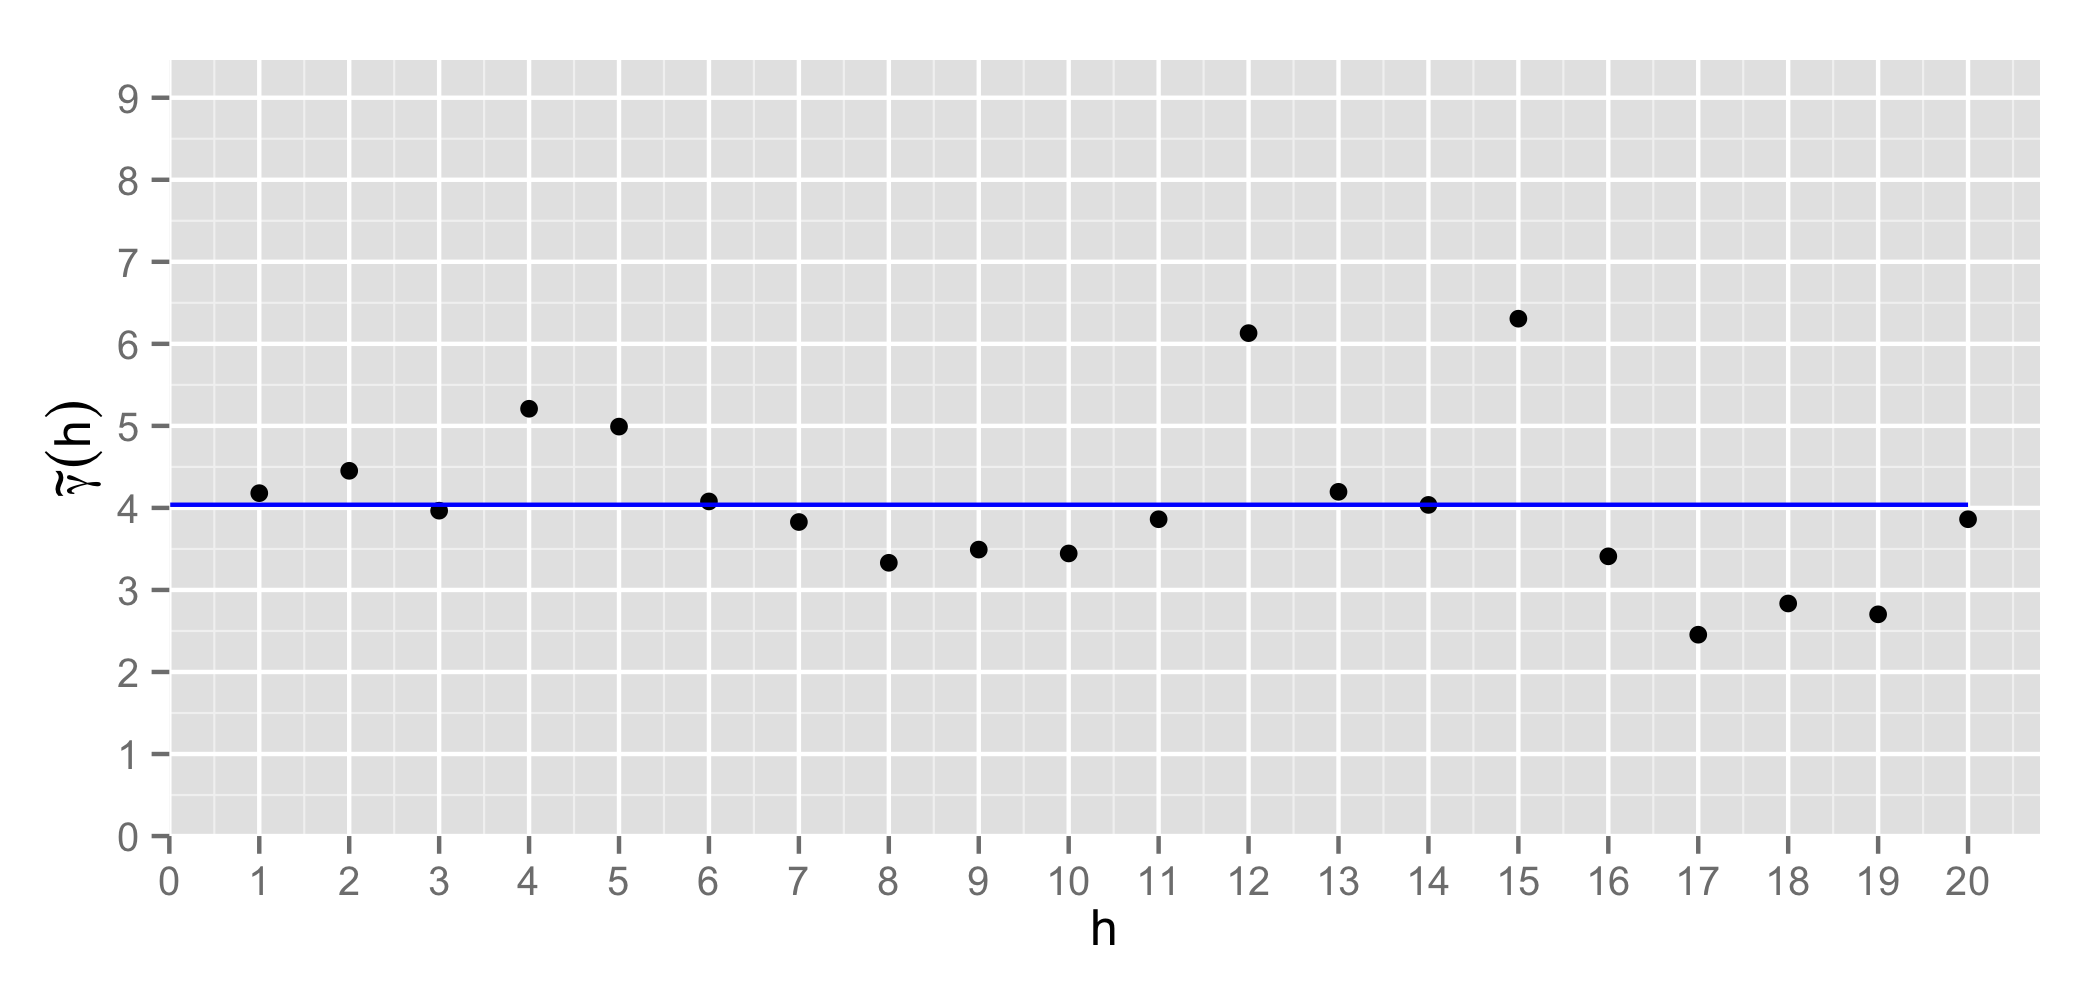
\includegraphics[width=0.8\linewidth]{../figures/variogram/lin-fit-modeled.png}}
\caption{Семивариограмма и оценка $ \widehat{\gamma}_2(h) $}
\label{img:lin-fit}
\end{figure}

\begin{figure}[H]
	\center{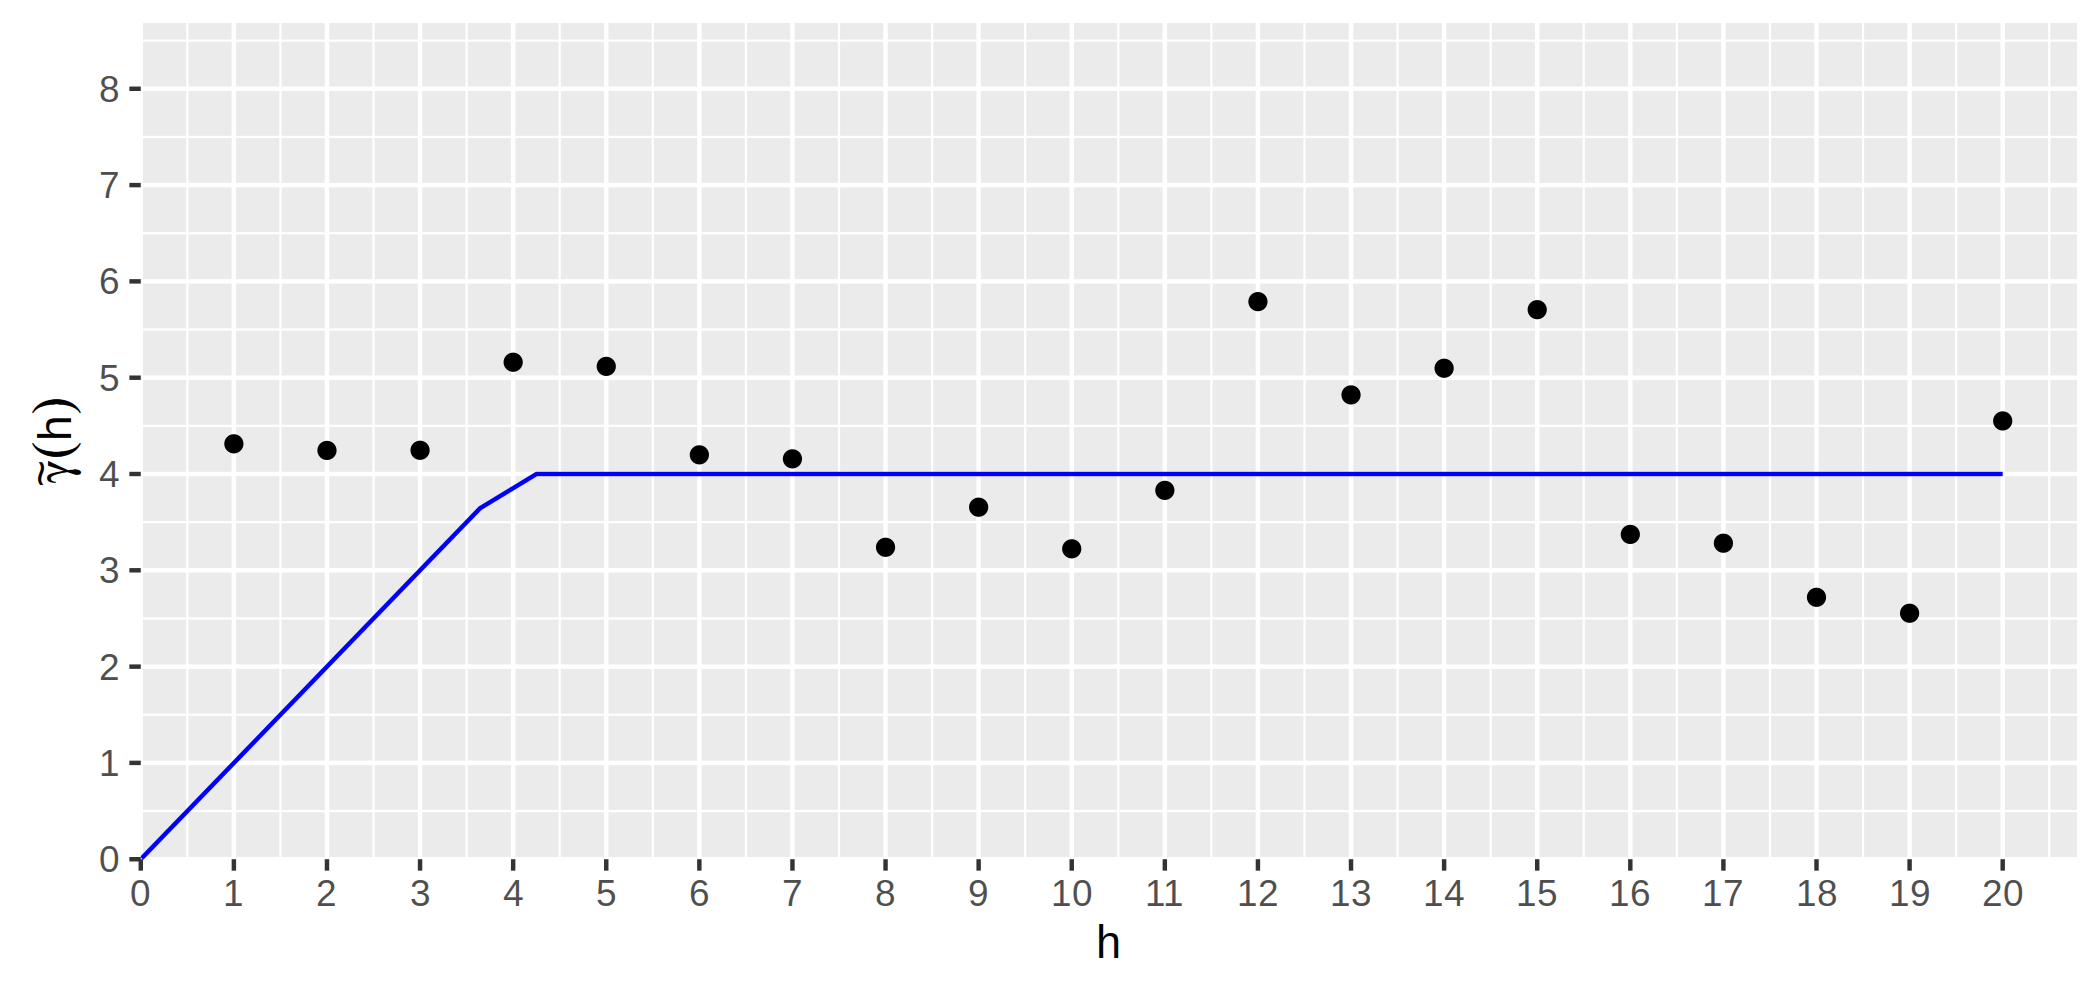
\includegraphics[width=0.8\linewidth]{../figures/variogram/lin-fit-cv-modeled.png}}
\caption{Семивариограмма и оценка $ \widehat{\gamma}_3(h) $}
\label{img:lin-fit-cv}
\end{figure}

\begin{figure}[H]
	\center{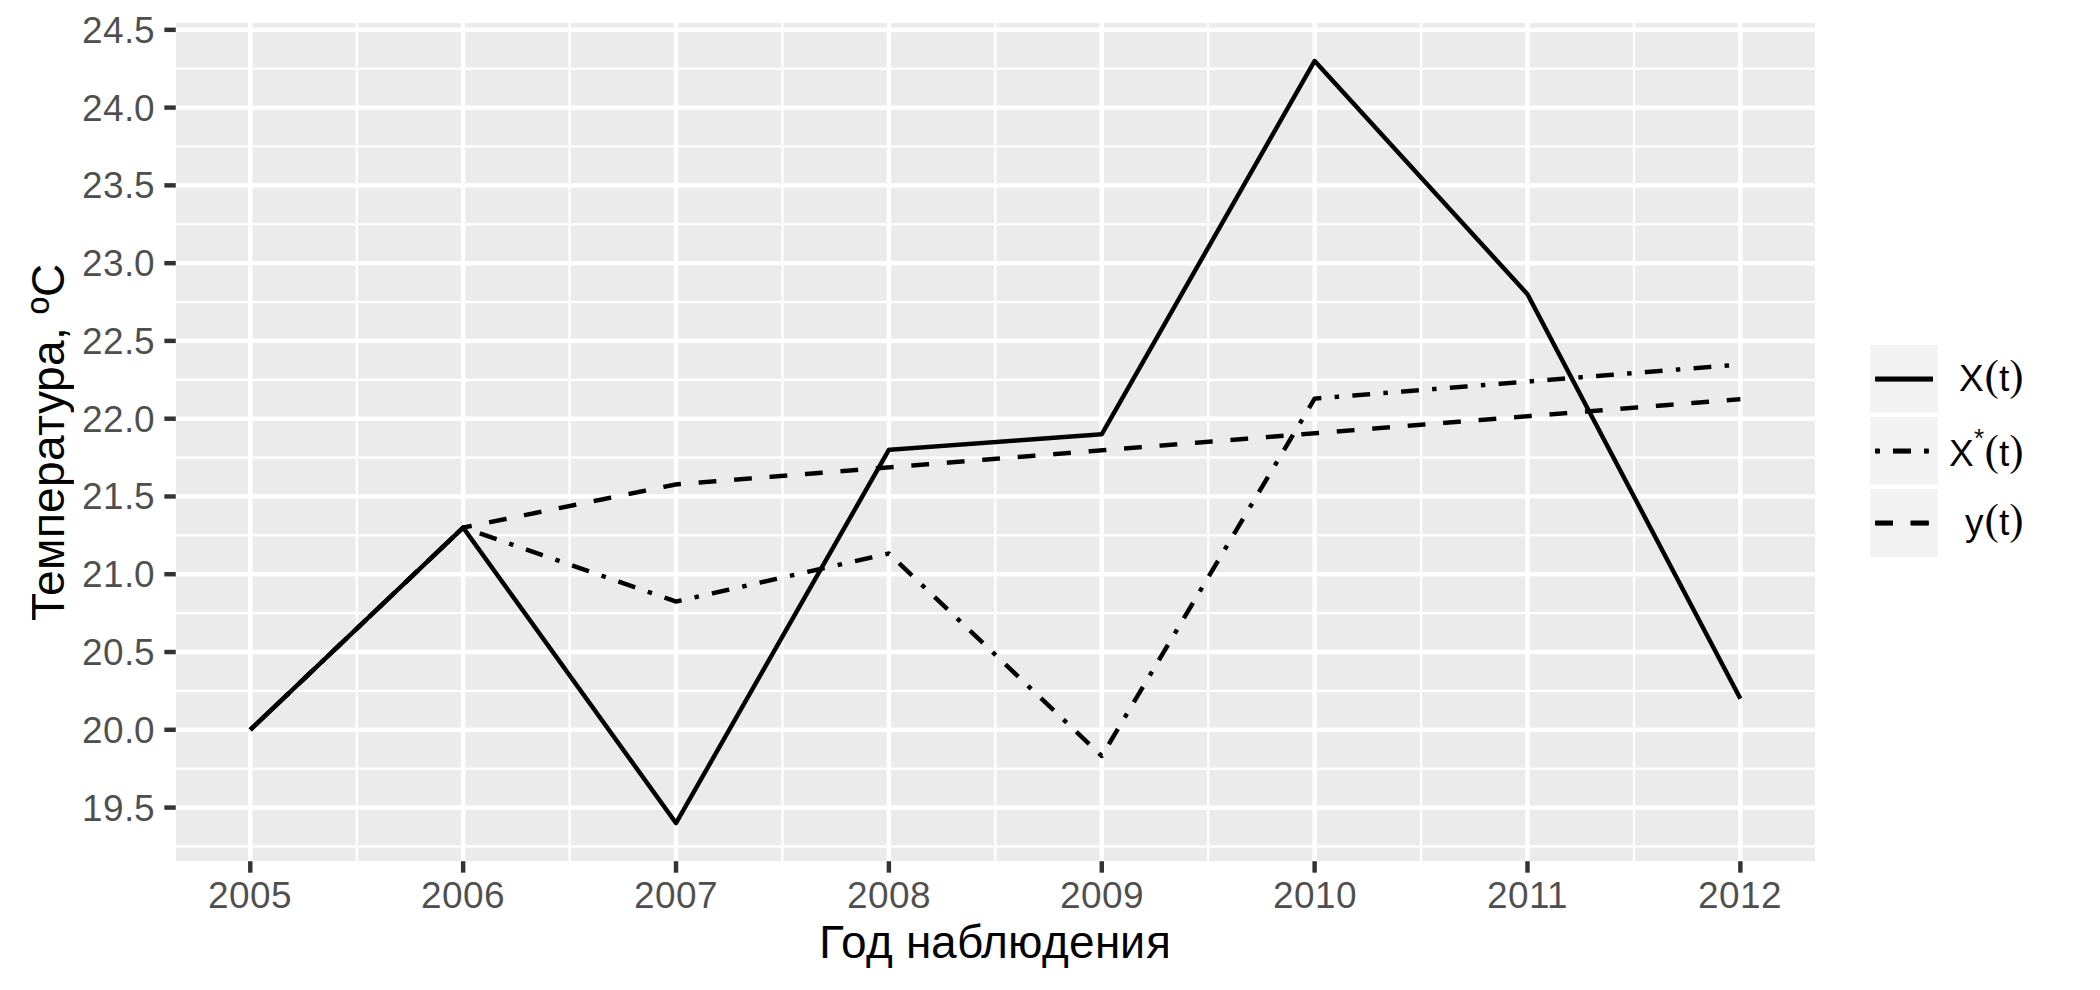
\includegraphics[width=0.8\linewidth]{../figures/variogram/lin-fit-cv-cross-prediction.png}}
\caption{Прогноз (модель $ \widehat{\gamma}_3(h) $)}
\label{img:lin-fit-cv-pred}
\end{figure}

\begin{figure}[H]
	\center{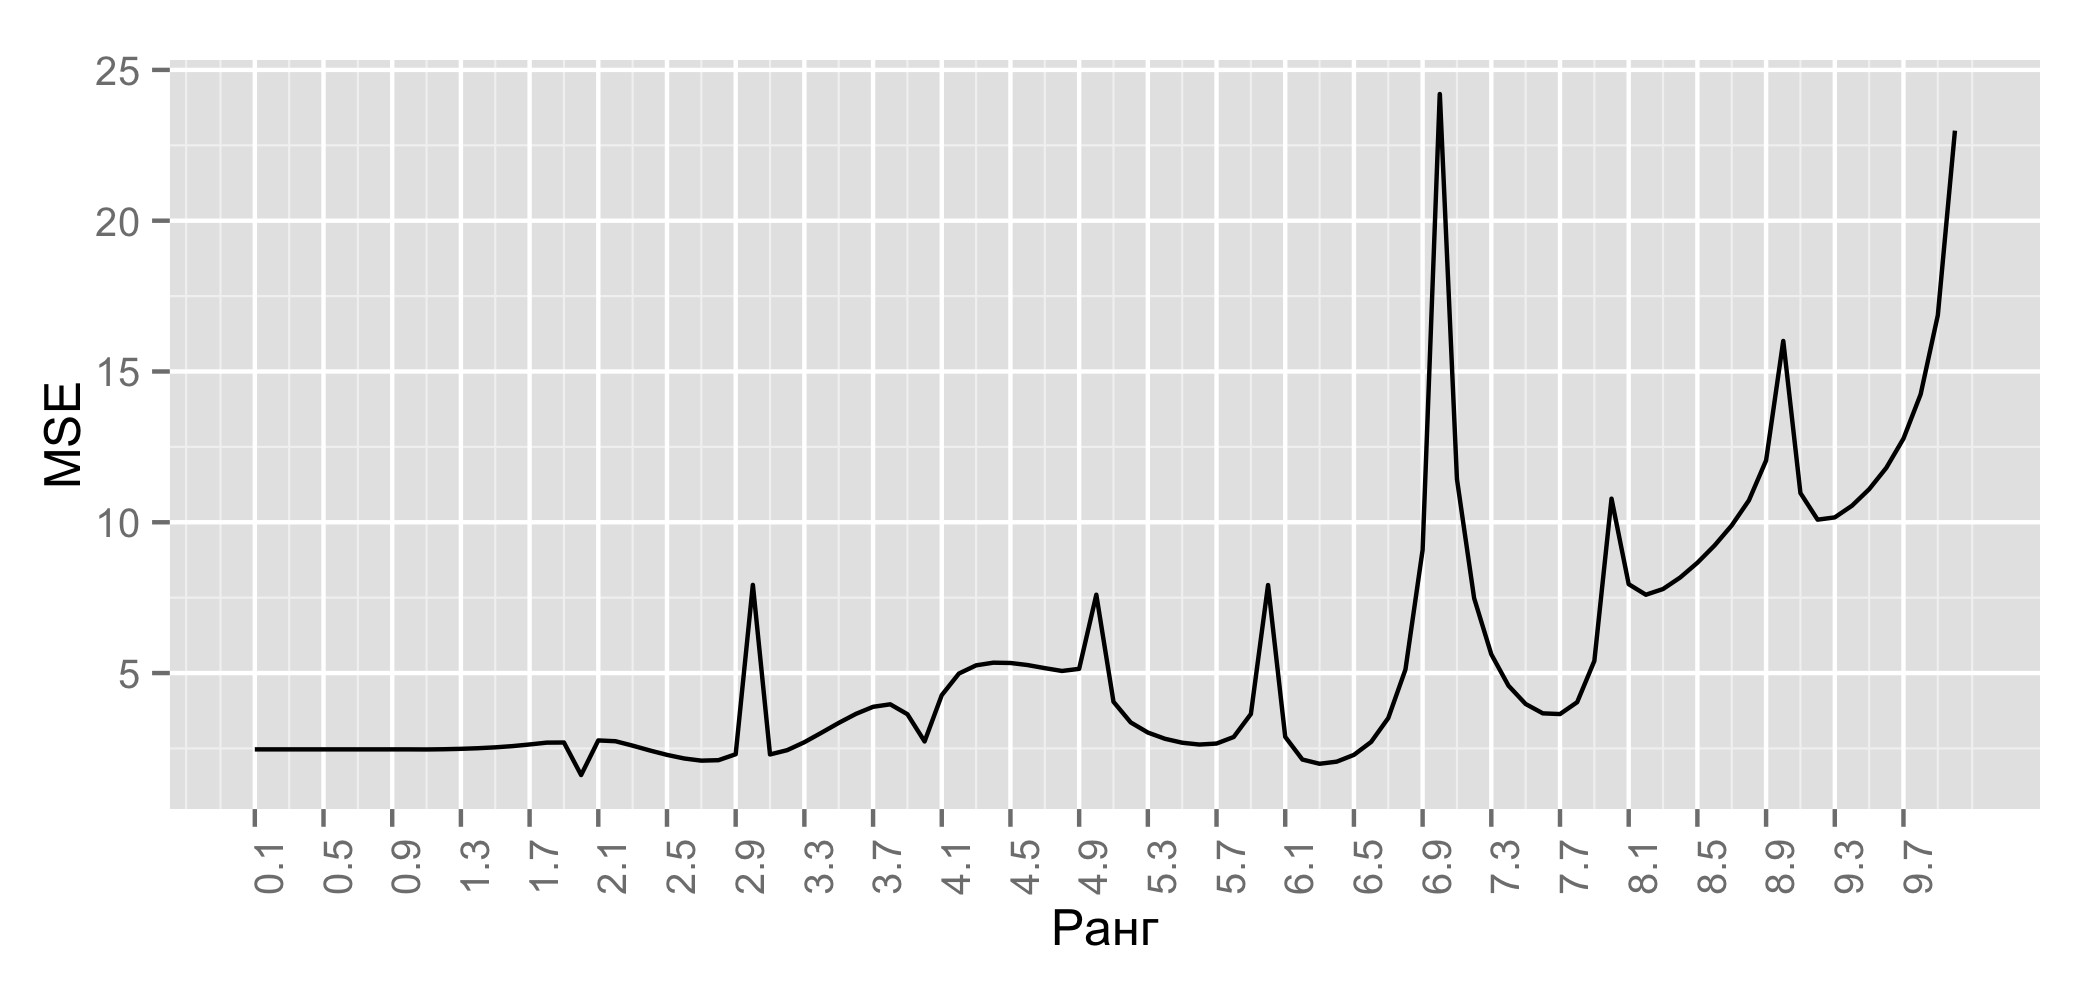
\includegraphics[width=0.8\linewidth]{../figures/variogram/lin-range-adapt.png}}
\caption{Зависимость качества линейной модели от значения ранга}
\label{img:lin-range-adapt}
\end{figure}

\begin{figure}[H]
	\center{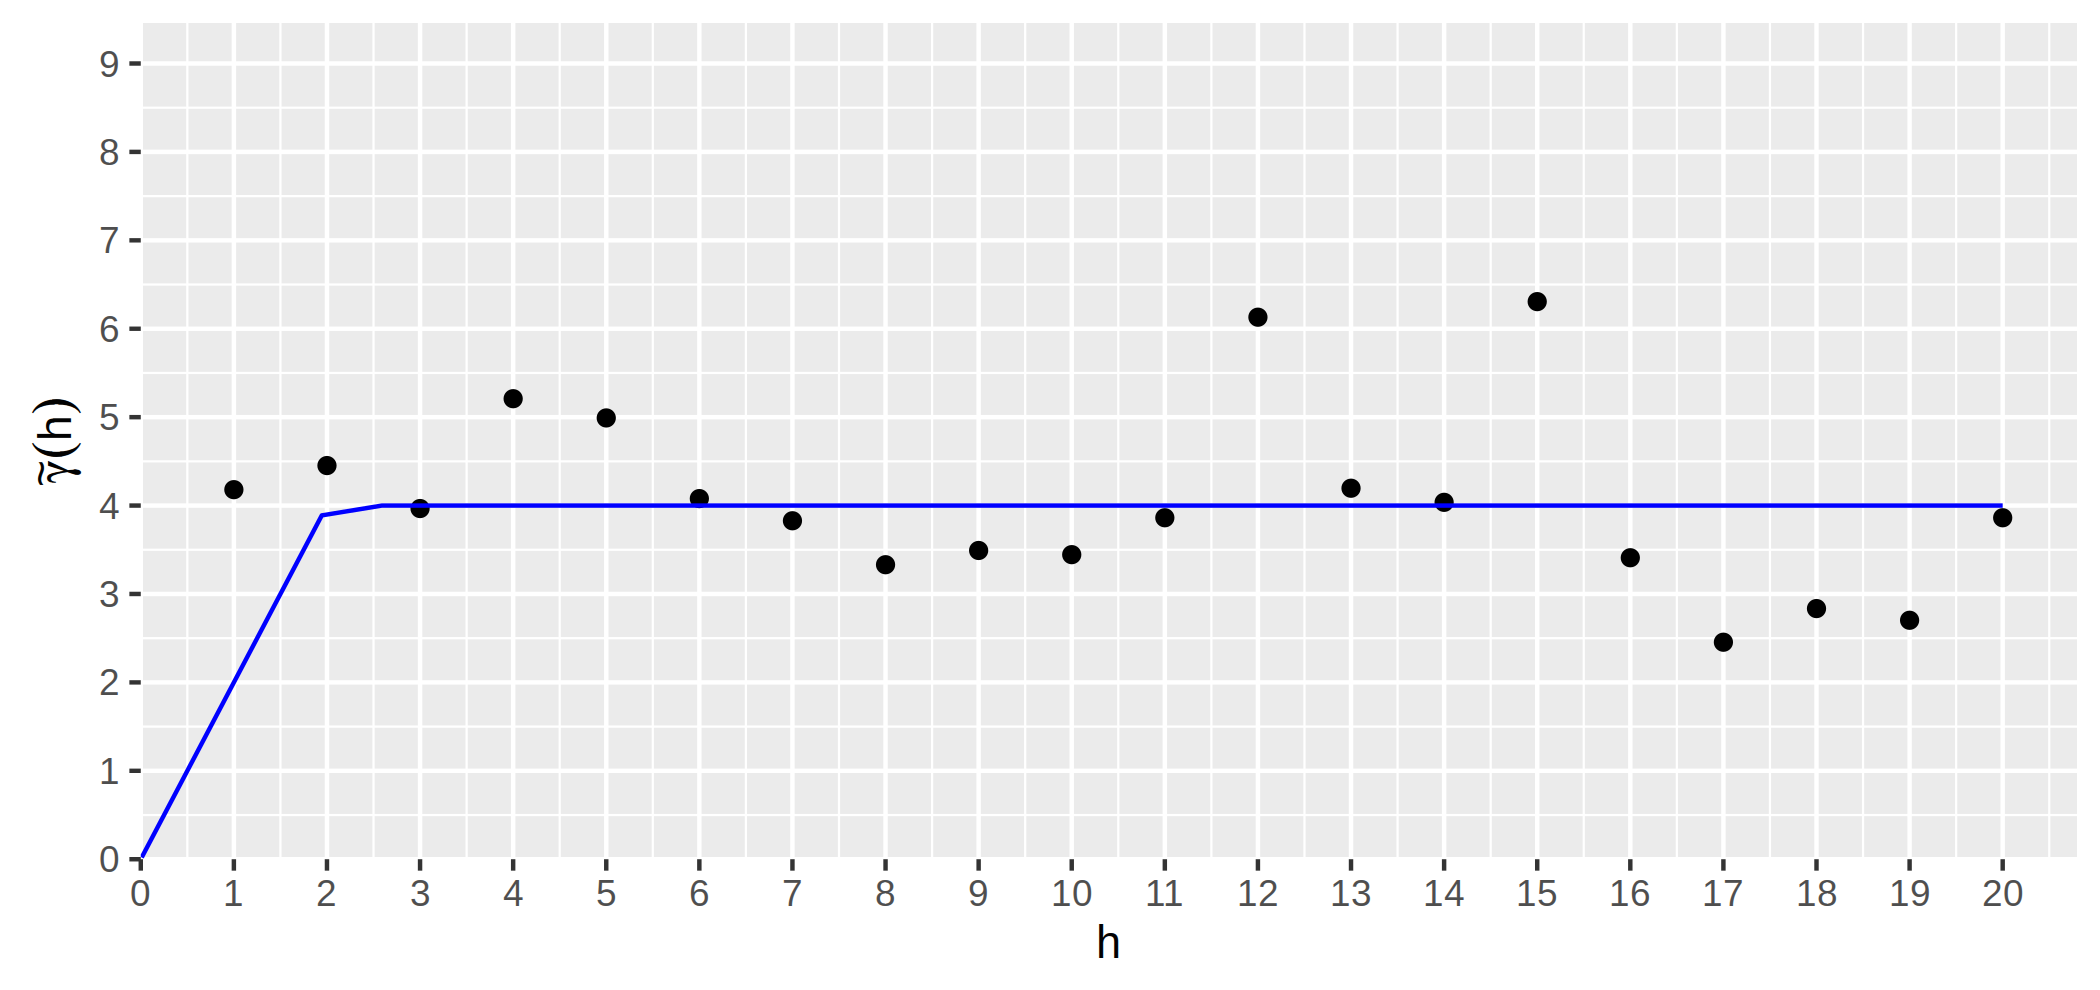
\includegraphics[width=0.8\linewidth]{../figures/variogram/lin-fit-adapt-modeled.png}}
\caption{Семивариограмма и оценка $ \widehat{\gamma}_4(h) $}
\label{img:lin-adapt-modeled}
\end{figure}

\begin{figure}[H]
	\center{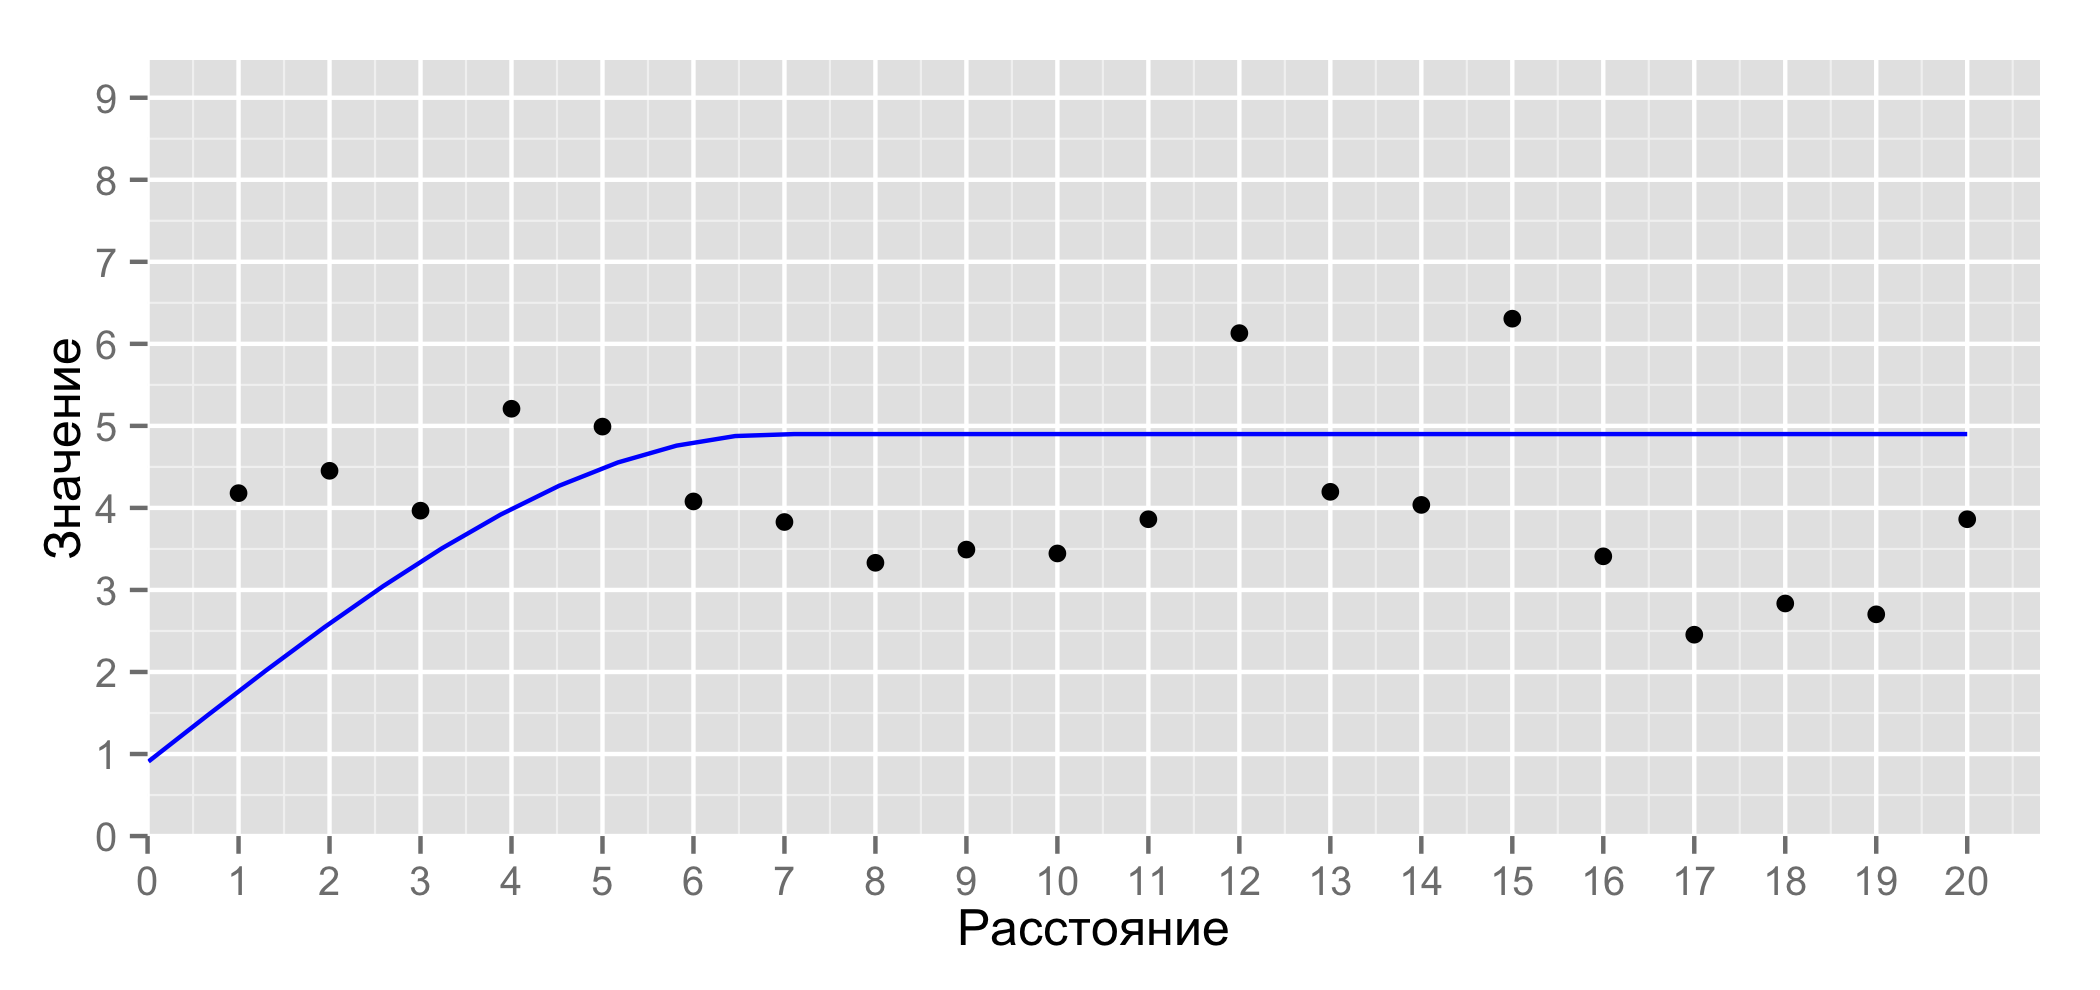
\includegraphics[width=0.8\linewidth]{../figures/variogram/sph-fit-adapt-modeled.png}}
\caption{Семивариограмма и оценка $ \widehat{\gamma}_5(h) $}
\label{img:sph-adapt-modeled}
\end{figure}

\begin{figure}[H]
	\center{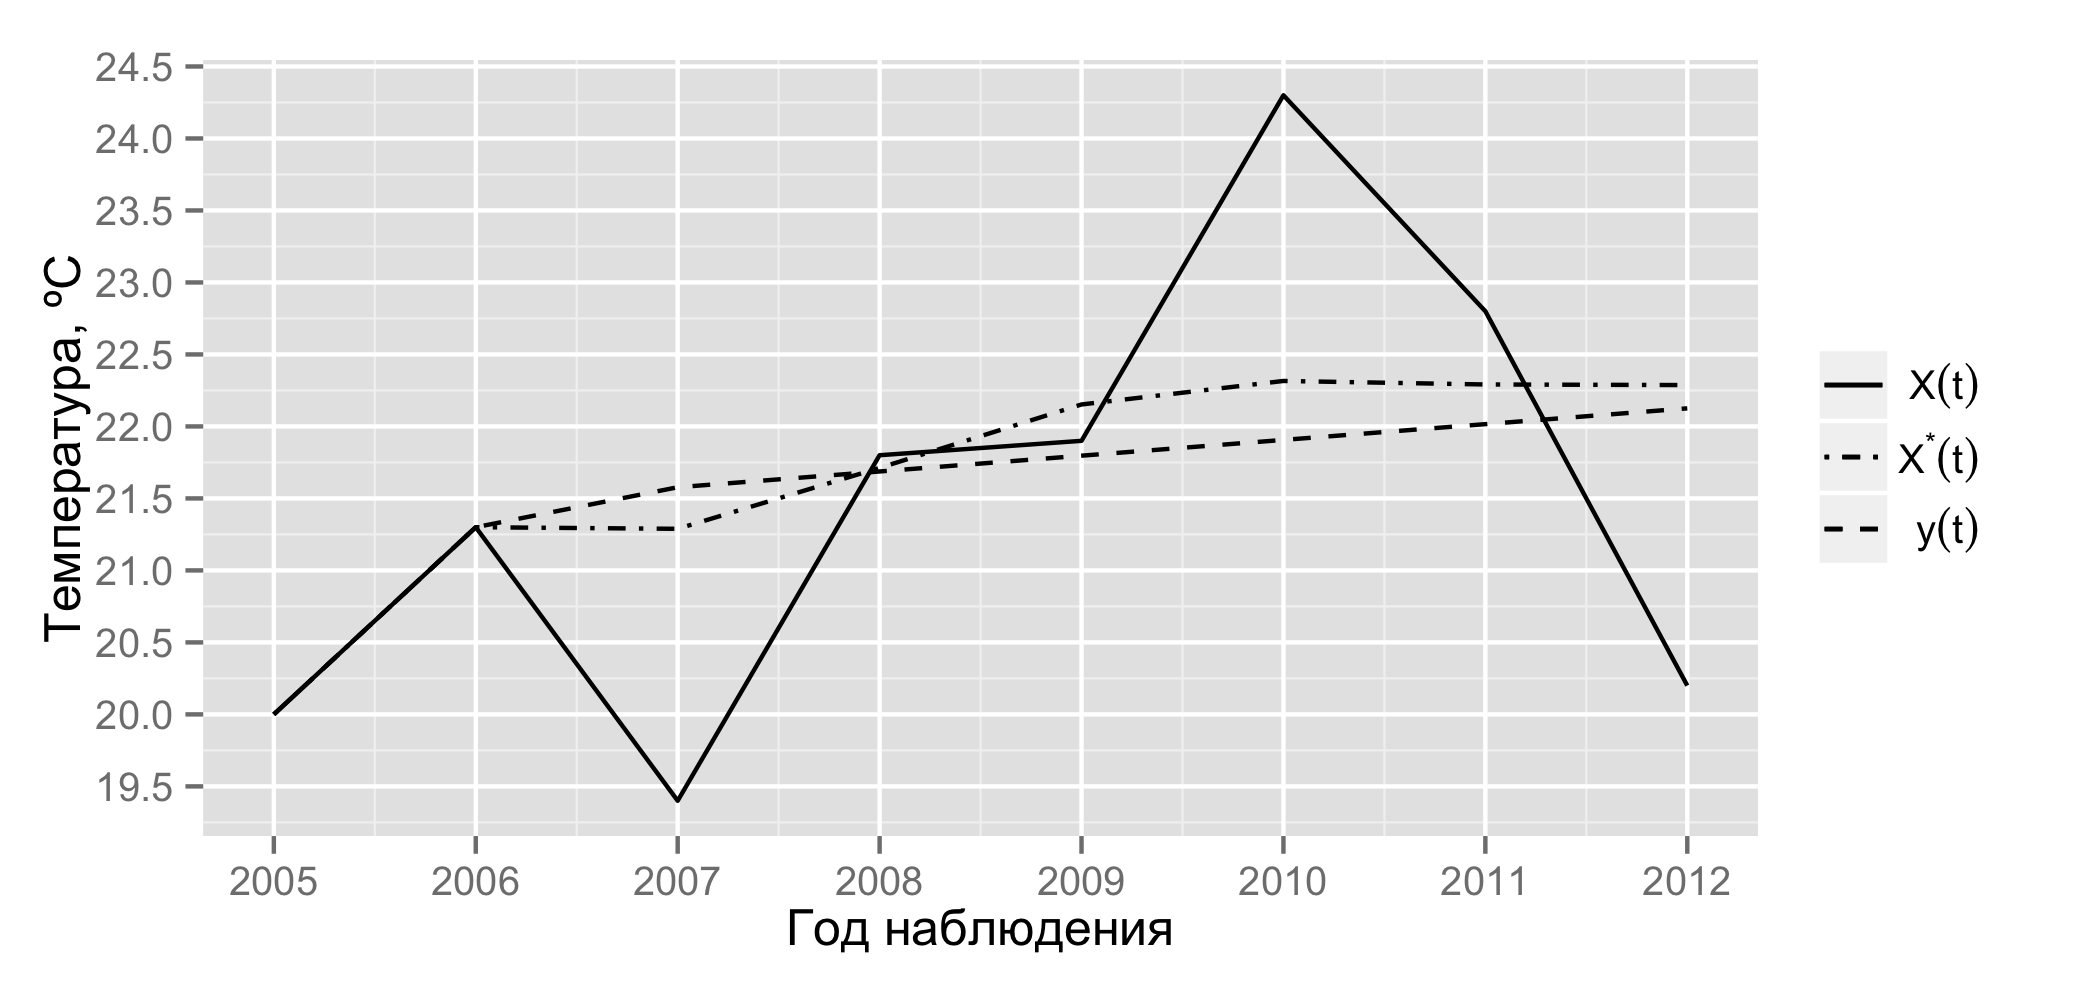
\includegraphics[width=0.8\linewidth]{../figures/variogram/sph-fit-adapt-cross-prediction.png}}
\caption{Прогноз (модель $ \widehat{\gamma}_5(h) $)}
\label{img:sph-adapt-pred}
\end{figure}

\begin{figure}[H]
	\center{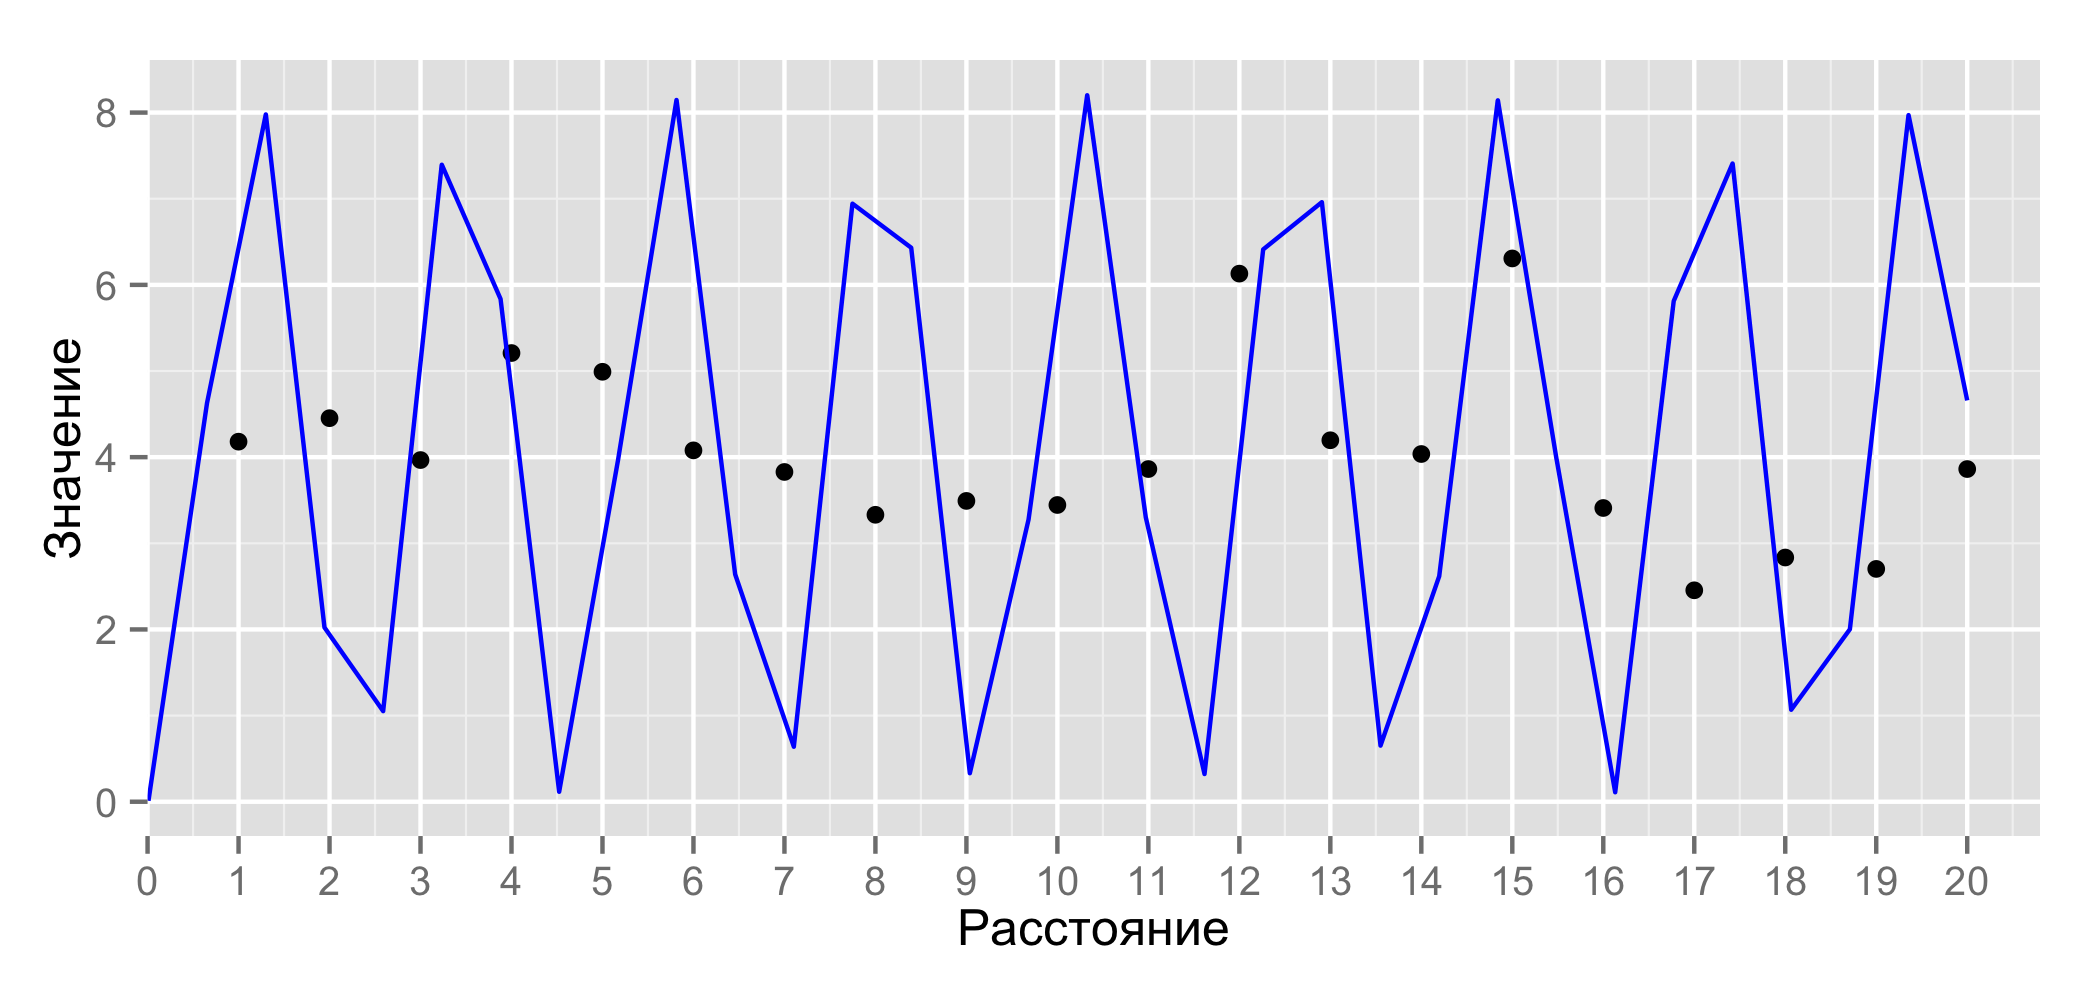
\includegraphics[width=0.8\linewidth]{../figures/variogram/per-fit-cv-modeled.png}}
\caption{Семивариограмма и оценка $ \widehat{\gamma}_6(h) $}
\label{img:per-cv-modeled}
\end{figure}

\begin{figure}[H]
\center{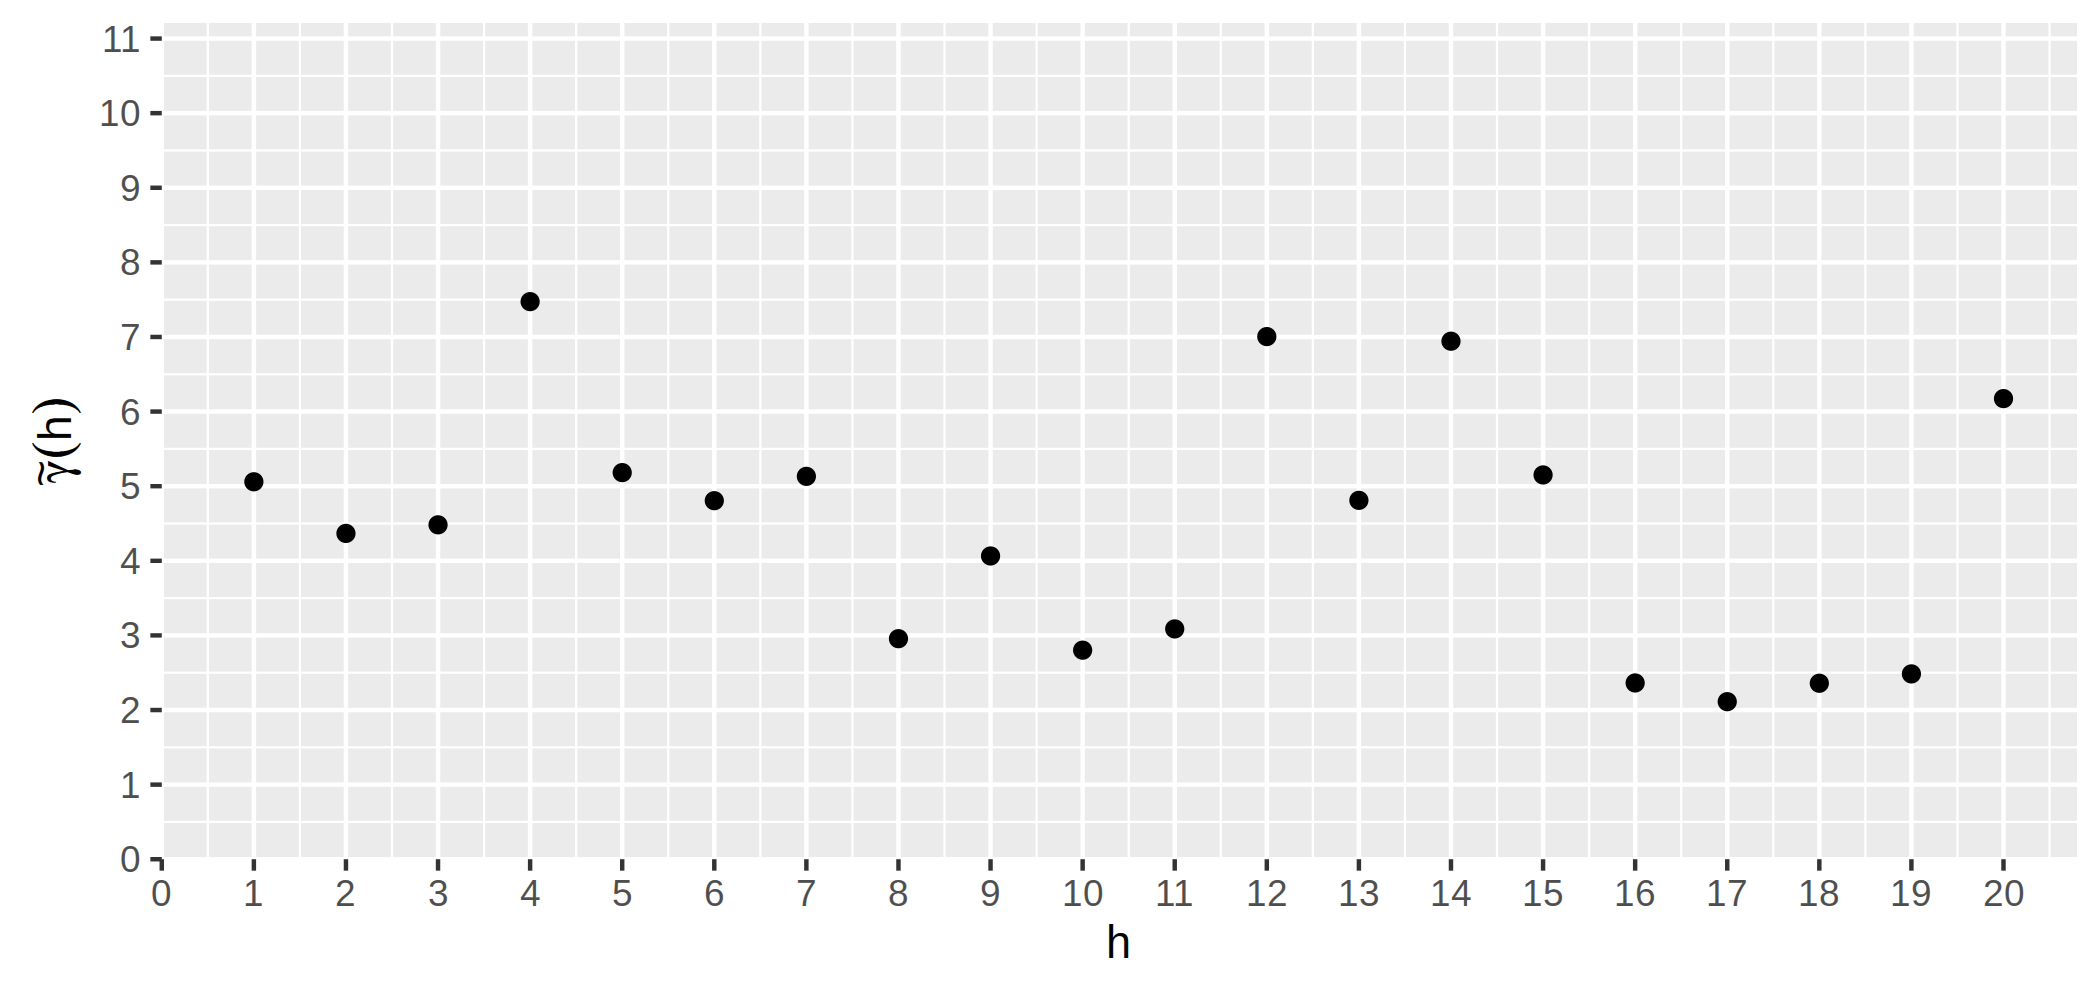
\includegraphics[width=0.8\linewidth]{../figures/variogram/robust-variogram.png}}
\caption{Оценка семивариограммы Кресси-Хокинса}
\label{img:robust-variogram}
\end{figure}

\begin{figure}[H]
\center{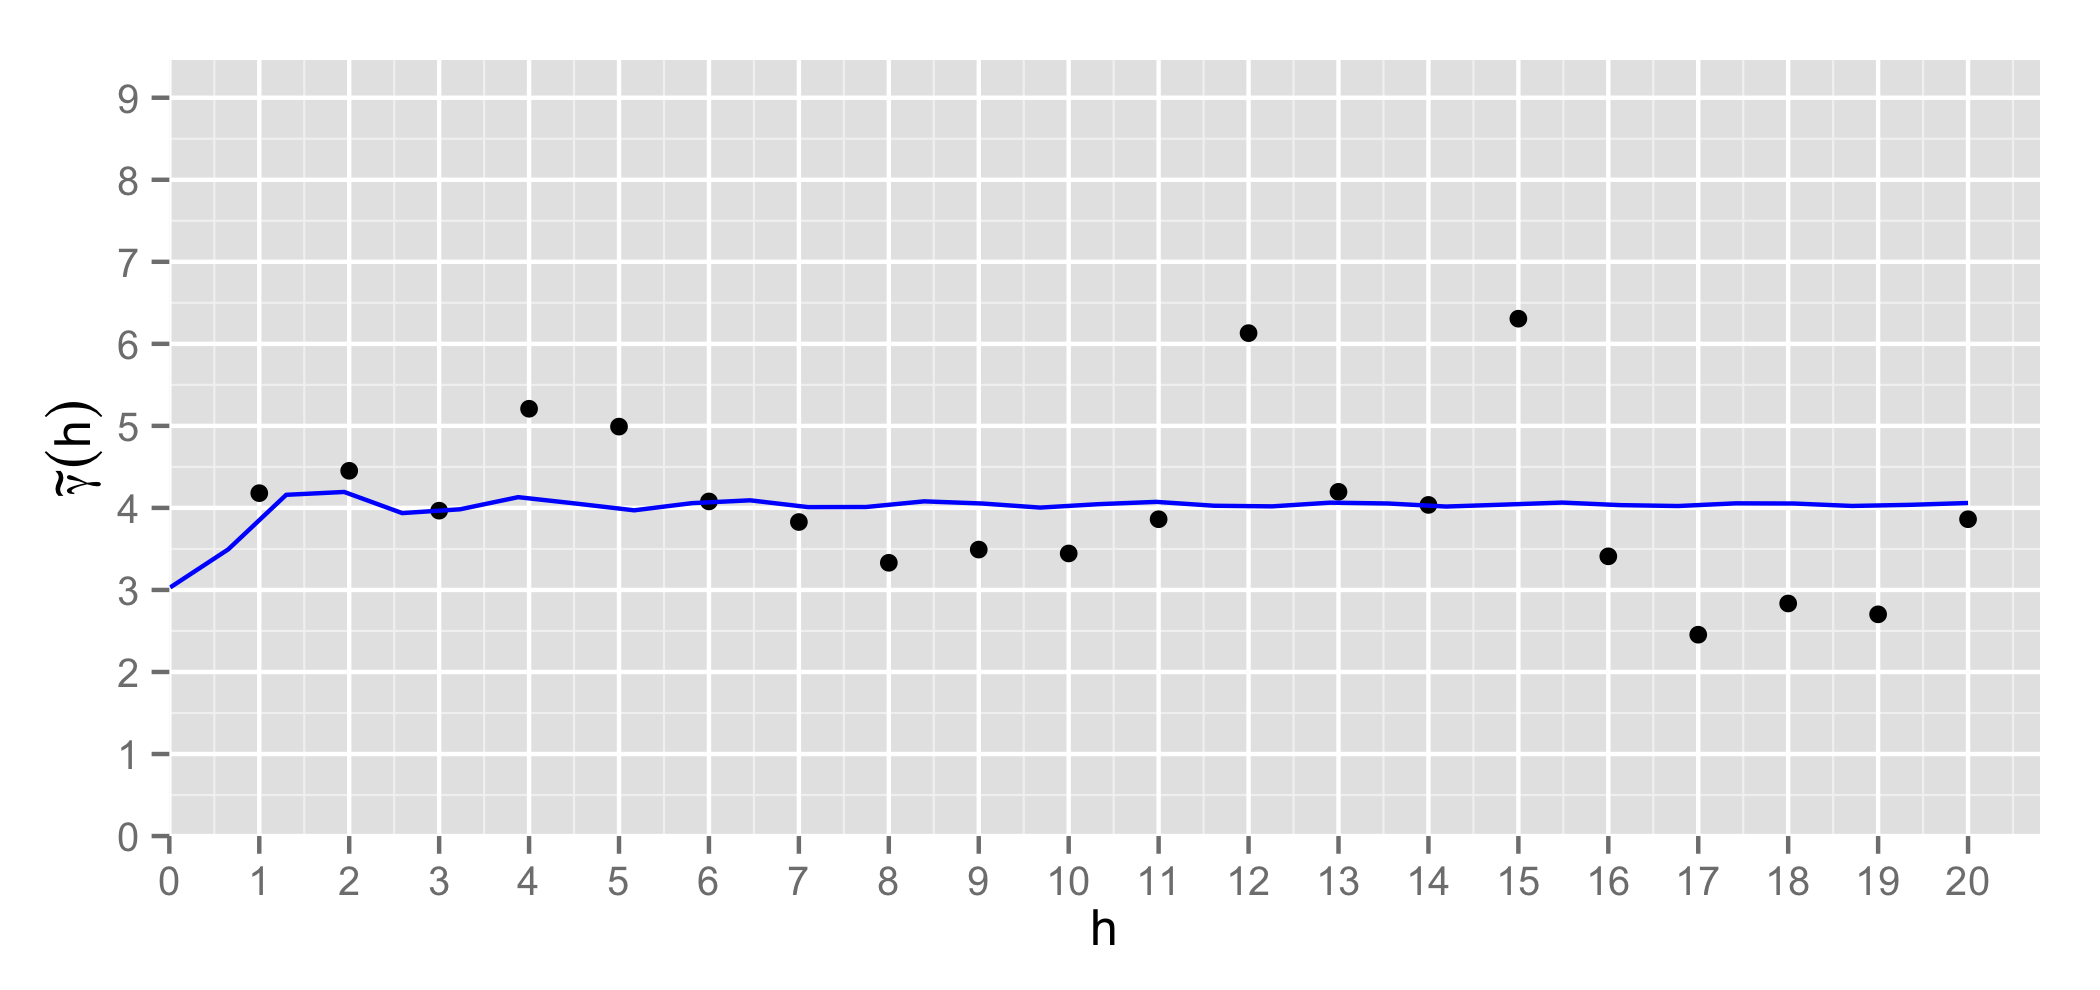
\includegraphics[width=0.8\linewidth]{../figures/variogram/auto-class-20-modeled.png}}
\caption{Семивариограмма и оценка $ \widehat{\gamma}_7(h) $}
\label{img:auto-class-modeled}
\end{figure}

\begin{figure}[H]
\center{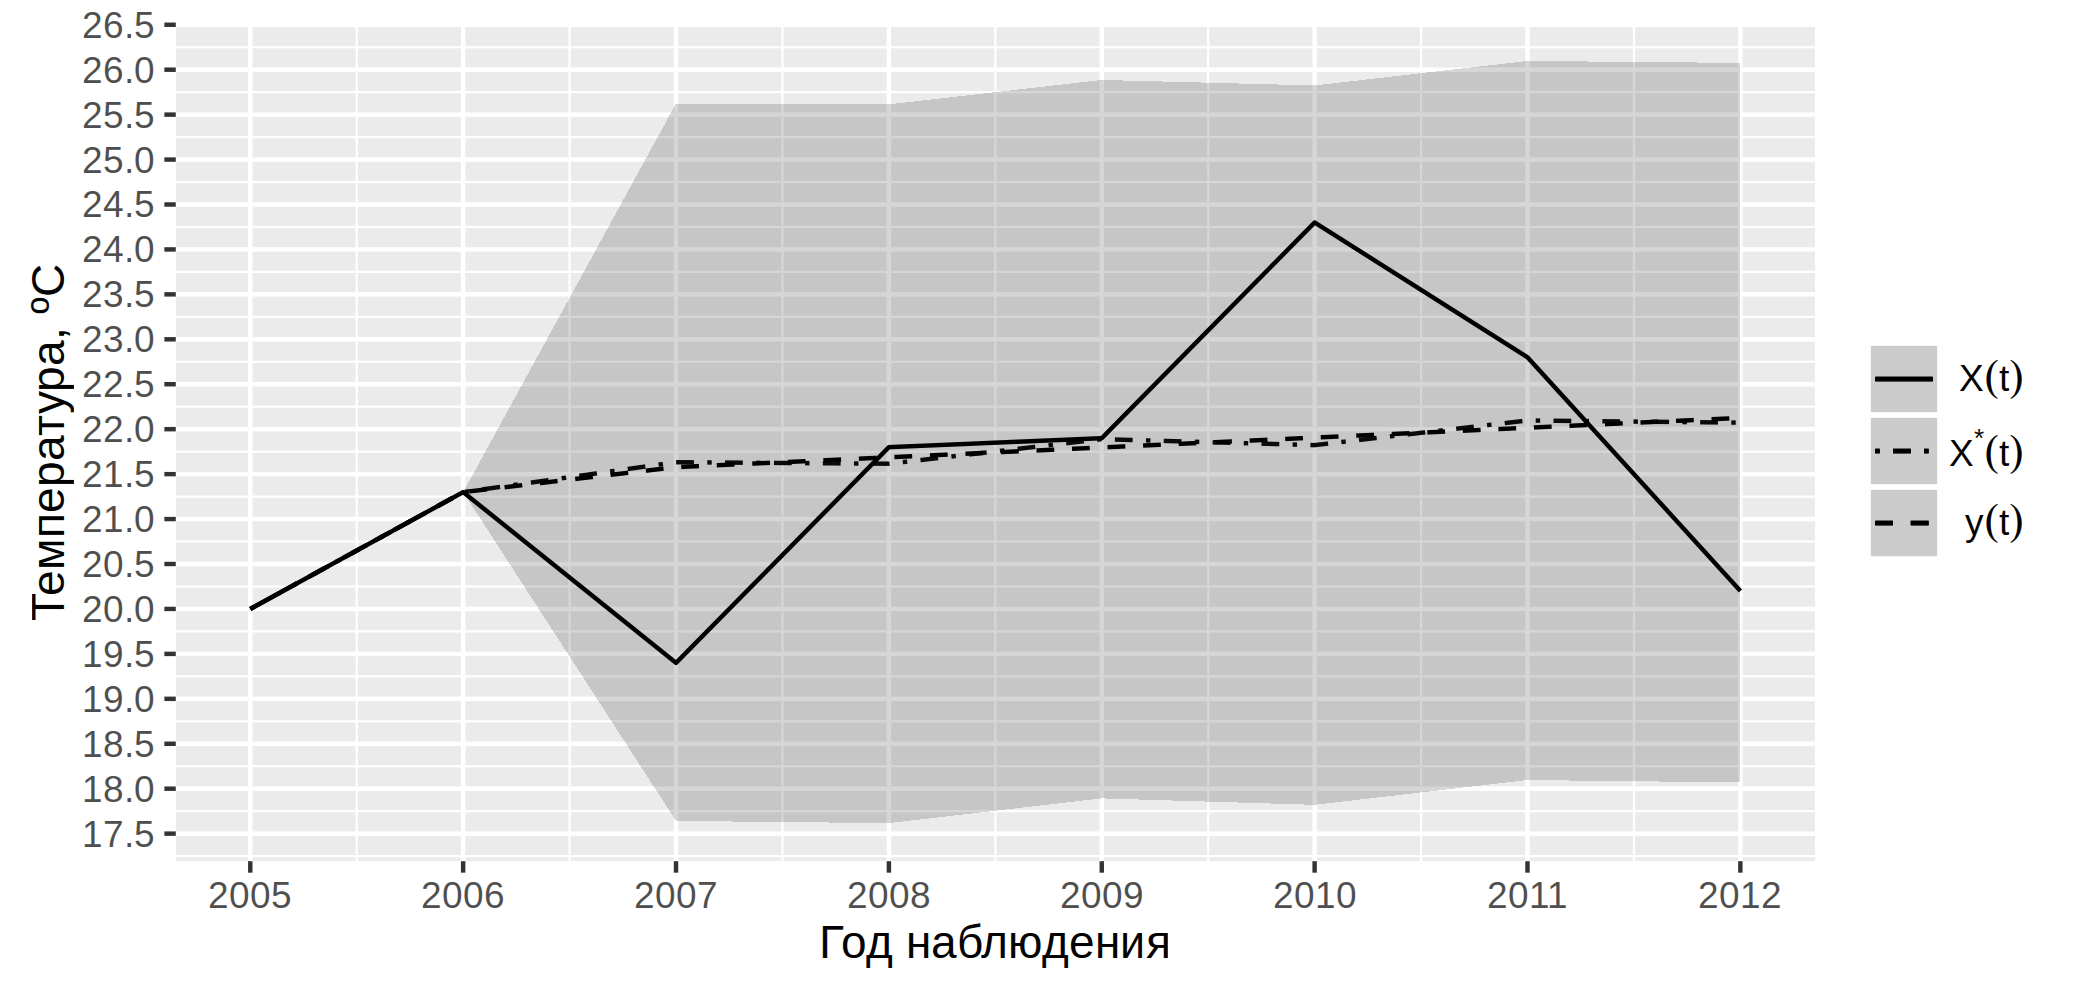
\includegraphics[width=0.8\linewidth]{../figures/variogram/auto-class-20-cross-prediction.png}}
\caption{Прогноз (модель $ \widehat{\gamma}_7(h) $)}
\label{img:auto-class-20-pred}
\end{figure}

\begin{figure}[H]
\center{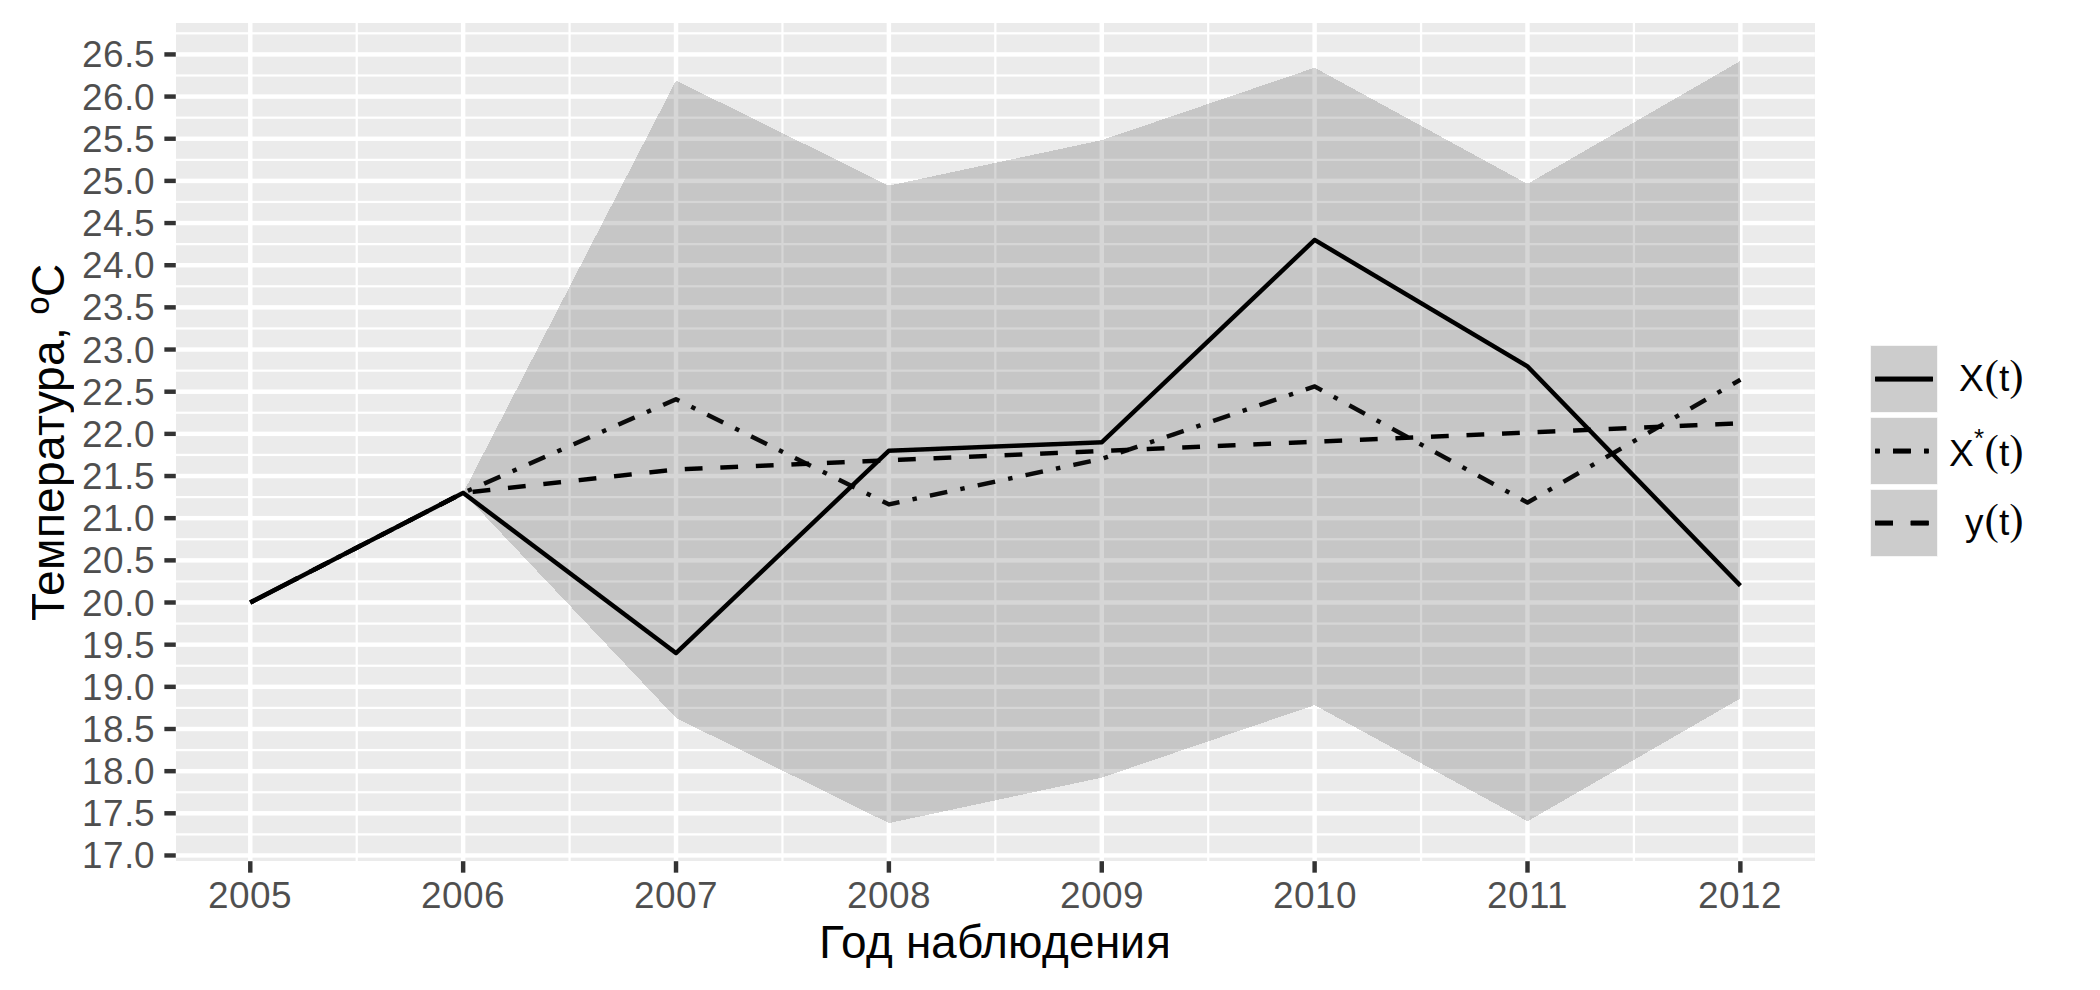
\includegraphics[width=0.8\linewidth]{../figures/variogram/auto-class-26-cross-prediction.png}}
\caption{Прогноз (модель $ \widehat{\gamma}_8(h) $)}
\label{img:auto-class-26-pred}
\end{figure}

\begin{figure}[H]
\center{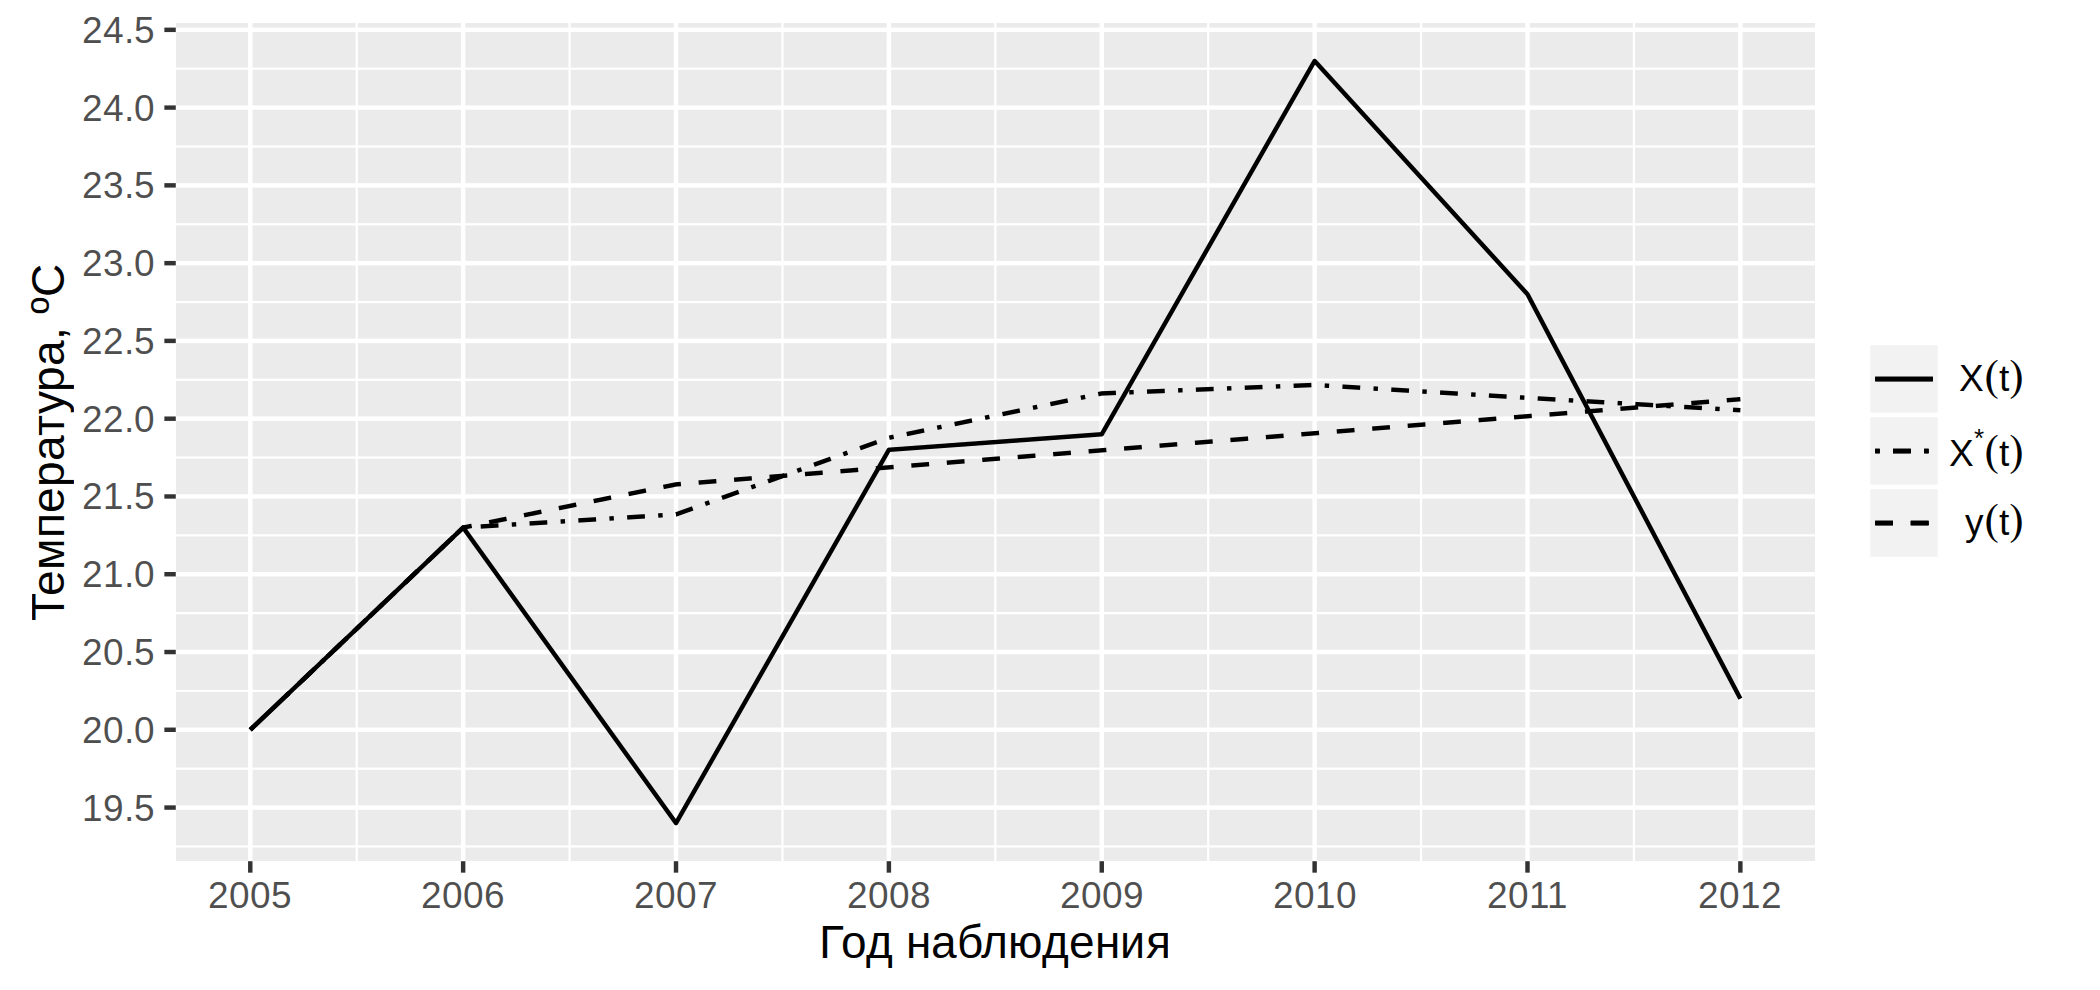
\includegraphics[width=0.8\linewidth]{../figures/variogram/auto-rob-5-cross-prediction.png}}
\caption{Прогноз (модель $ \widehat{\gamma}_9(h) $)}
\label{img:auto-rob-5-pred}
\end{figure}

\begin{figure}[H]
\center{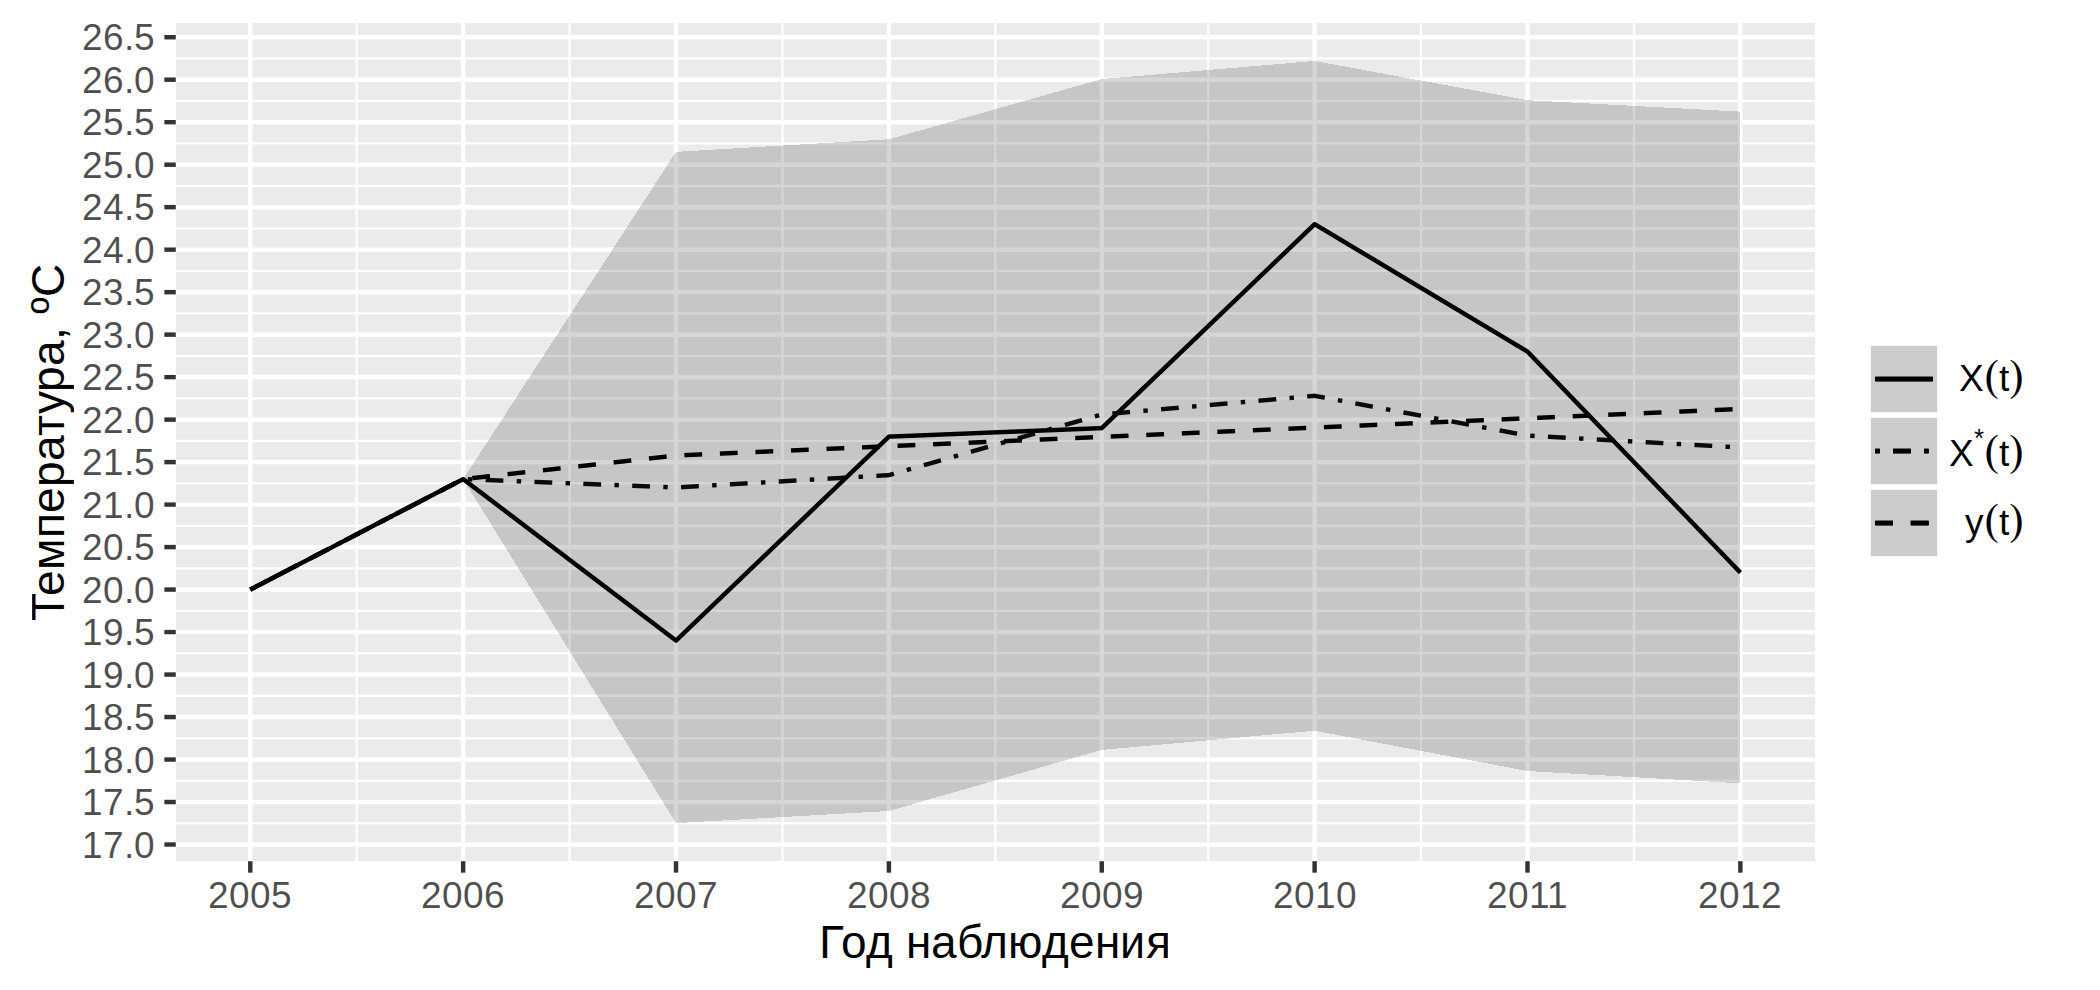
\includegraphics[width=0.8\linewidth]{../figures/variogram/auto-class-18-cross-prediction.png}}
\caption{Прогноз (модель $ \widehat{\gamma}_{10}(h) $)}
\label{img:auto-class-18-pred}
\end{figure}
